Como mencionado anteriormente, este trabalho tem como objetivo desenvolver o design de um circuito integrado para um DPD, partindo de um modelo previamente validado tanto em software quanto em hardware, especificamente em FPGA. O projeto foi dividido em quatro etapas principais:

\begin{itemize}
\item Estudo do DPD;
\item Implementação em software;
\item Implementação em FPGA;
\item Design e validação do circuito integrado.
\end{itemize}


\section{Estudo dos DPDs}
A etapa consistiu no estudo dos DPDs, conforme apresentado no Capítulo \ref{chap:revi}, onde foi feito todo o levantamento sobre os tipos de modelagem dos DPDs. O objetivo deste estudo é entender as diferentes abordagens de modelagem, avaliar seus desempenhos e identificar as mais adequadas para a aplicação em amplificadores de potência.

\section{Implementação em software} \label{sec:implsoft}

Nesta etapa, foi realizada a implementação do modelo DPD em software, utilizando a linguagem de programação Python. Esta linguagem amigável e amplamente difundida na comunidade acadêmica.

Para essa modelagem, foram coletados sinais de entrada e saída de um amplificador de potência classe AB, que utiliza um HEMT fabricado com tecnologia GaN. O amplificador foi excitado por um sinal portador de frequência de 900 MHz, modulado por um sinal de envelope WCDMA 3GPP com aproximadamente 3,84 MHz de largura de banda. Os dados de entrada e saída do amplificador de potência foram medidos usando um VSA Rohde \& Schwarz FSQ com uma taxa de amostragem de 61,44 MHz, conforme disponível em \cite{Bonfim2016}.

Em seguida, realizou-se o cálculo da estimativa do sinal utilizando números com vírgula fixa. Para verificar a precisão dessa estimativa em relação ao sinal original, calculou-se o NMSE. Para essa validação, os dados foram inicialmente divididos em conjuntos de extração e validação. A matriz de extração foi calculada com os dados de extração, utilizando o código disponível no anexo \ref{cod:mp}. Esse cálculo é essencial para a extração dos coeficientes do polinômio de memória. Após a extração dos coeficientes, calculou-se o modelo do PA, que foi então validado com os dados de validação. O NMSE obtido para um polinômio de 2° grau com uma amostra memorizada foi de -23,57 dB.

Em seguida, o algoritmo foi ajustado para operar com números em vírgula fixa e o número total de bits foi reajustado para atingir a menor resolução possível, buscando o menor NMSE simulado, conforme ilustrado pelo anexo \ref{cod:mpint}. Por ser tratar de um cálculo em virgula fixa, fez-se necessário uma readequação do resultado obtido entre cada multiplicação de forma a manter a resolução inicial.

\section{Implementação em FPGA}
Essa etapa consiste na implementação do DPD em FPGA. Para isso, é necessário realizar paralelizações nas operações aritméticas. A Figura \ref{fig:diagramaprocess} ilustra como esse processo está dividido entre cada ciclo de clock. Aqui está o trecho reescrito de forma mais clara: A cada ciclo, duas operações são realizadas em paralelo: o sinal atual é elevado ao quadrado e registrado, enquanto ocorre o somatório do produto entre os sinais do mesmo instante de tempo e seus respectivos coeficientes. Esse processo ocorre P vezes para os \( P \) graus do polinômio de memória. Portanto, a saída do DPD é incompleta para os primeiros \( P \) períodos de clock, pois, nesses primeiros ciclos, realiza-se o cálculo com base em entradas de sinais anteriores que ainda não ocorreram, resultando em uma saída incompleta.

\begin{figure}[ht!]
  \centering
  \captionsetup{justification=centering}
  \caption*{Fonte: Autor}
  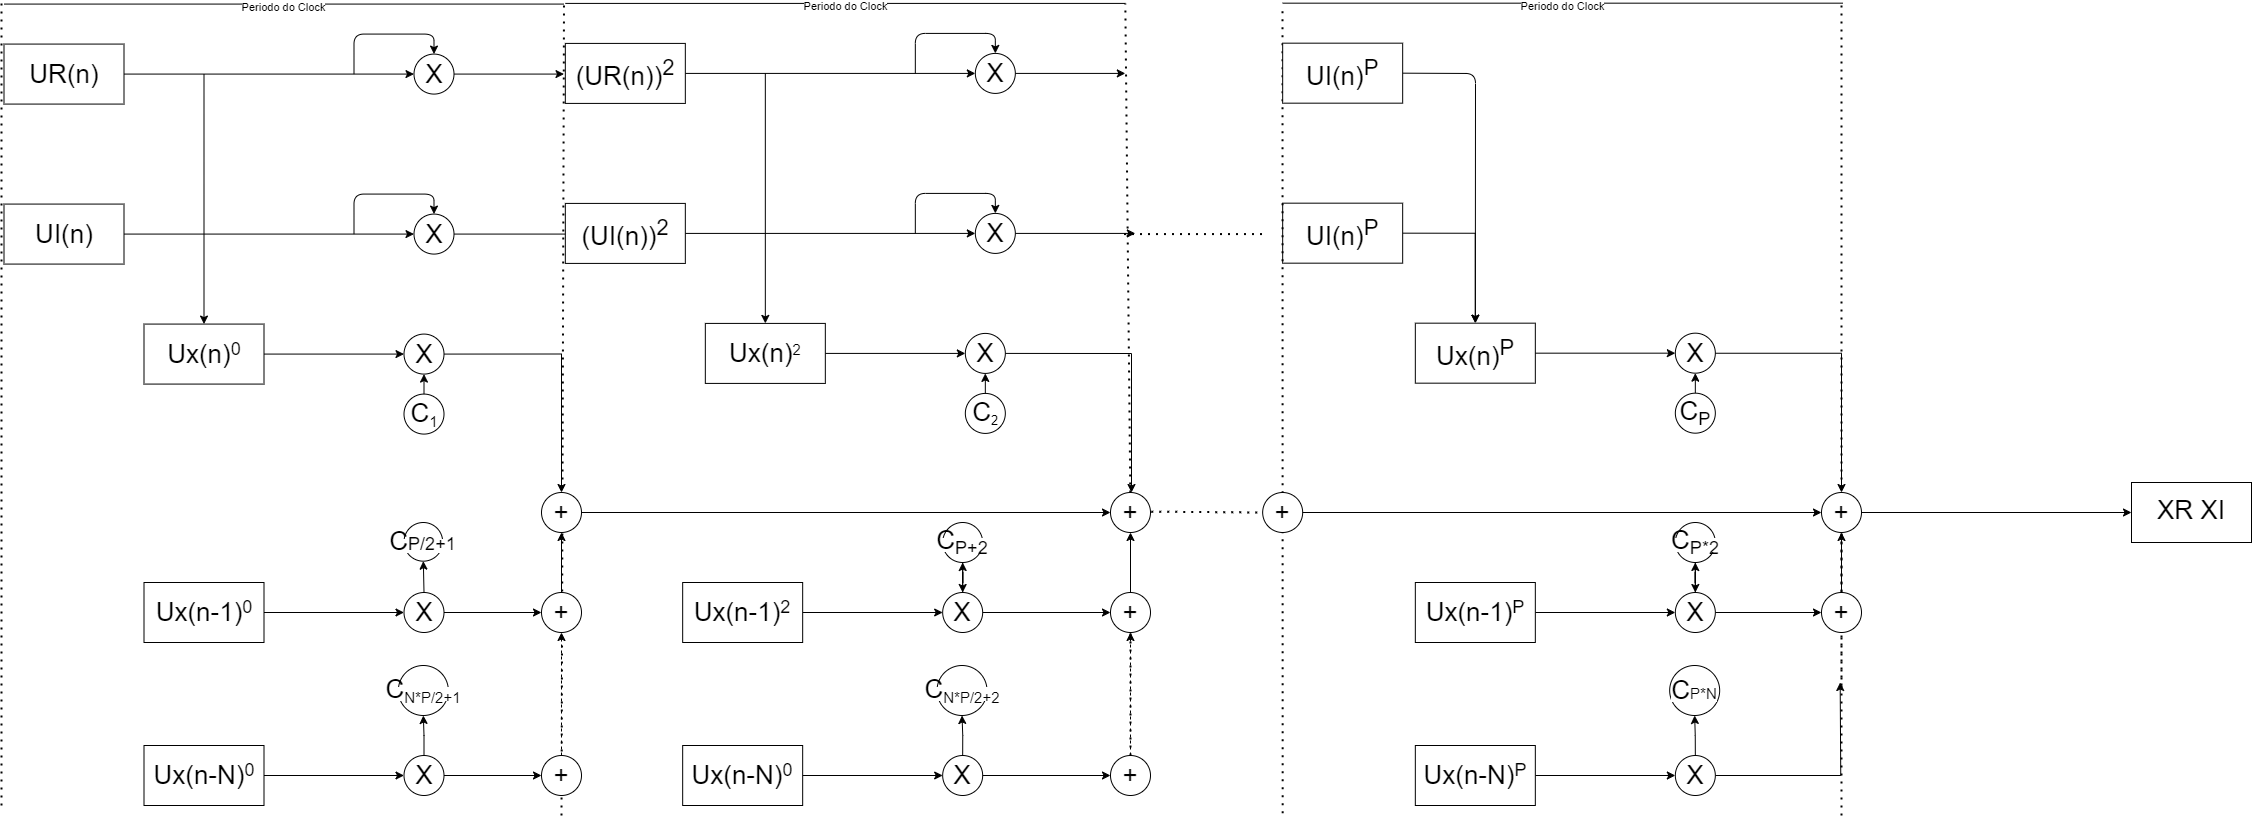
\includegraphics[width=0.80\textwidth]{diagrama_process.png}
  \caption{Processo de cálculo da saída}
  \label{fig:diagramaprocess}
\end{figure}

\section{Design e validação}
Finalmente, na última etapa, realiza-se o processo de concepção do circuito integrado do DPD como um circuito dedicado integrado na tecnologia BiCMOS 130 nm 8HP, utilizando as ferramentas específicas de desing de circuito integrado.
O fluxo de projeto VLSI para design de um circuito integrado de aplicação específica, inclui a descrição do circuito em VHDL, síntese lógica utilizando as células padrão da tecnologia, PAR (\textit{place and route}) e simulações comportamentais e temporais. O diagrama do fluxo VLSI pode ser ilustrado pela figura \ref{fig:CMOS2010}.

\begin{figure}[ht!]
  \centering
  \captionsetup{justification=centering}
  \caption*{Fonte: \cite{CMOS2010}}
  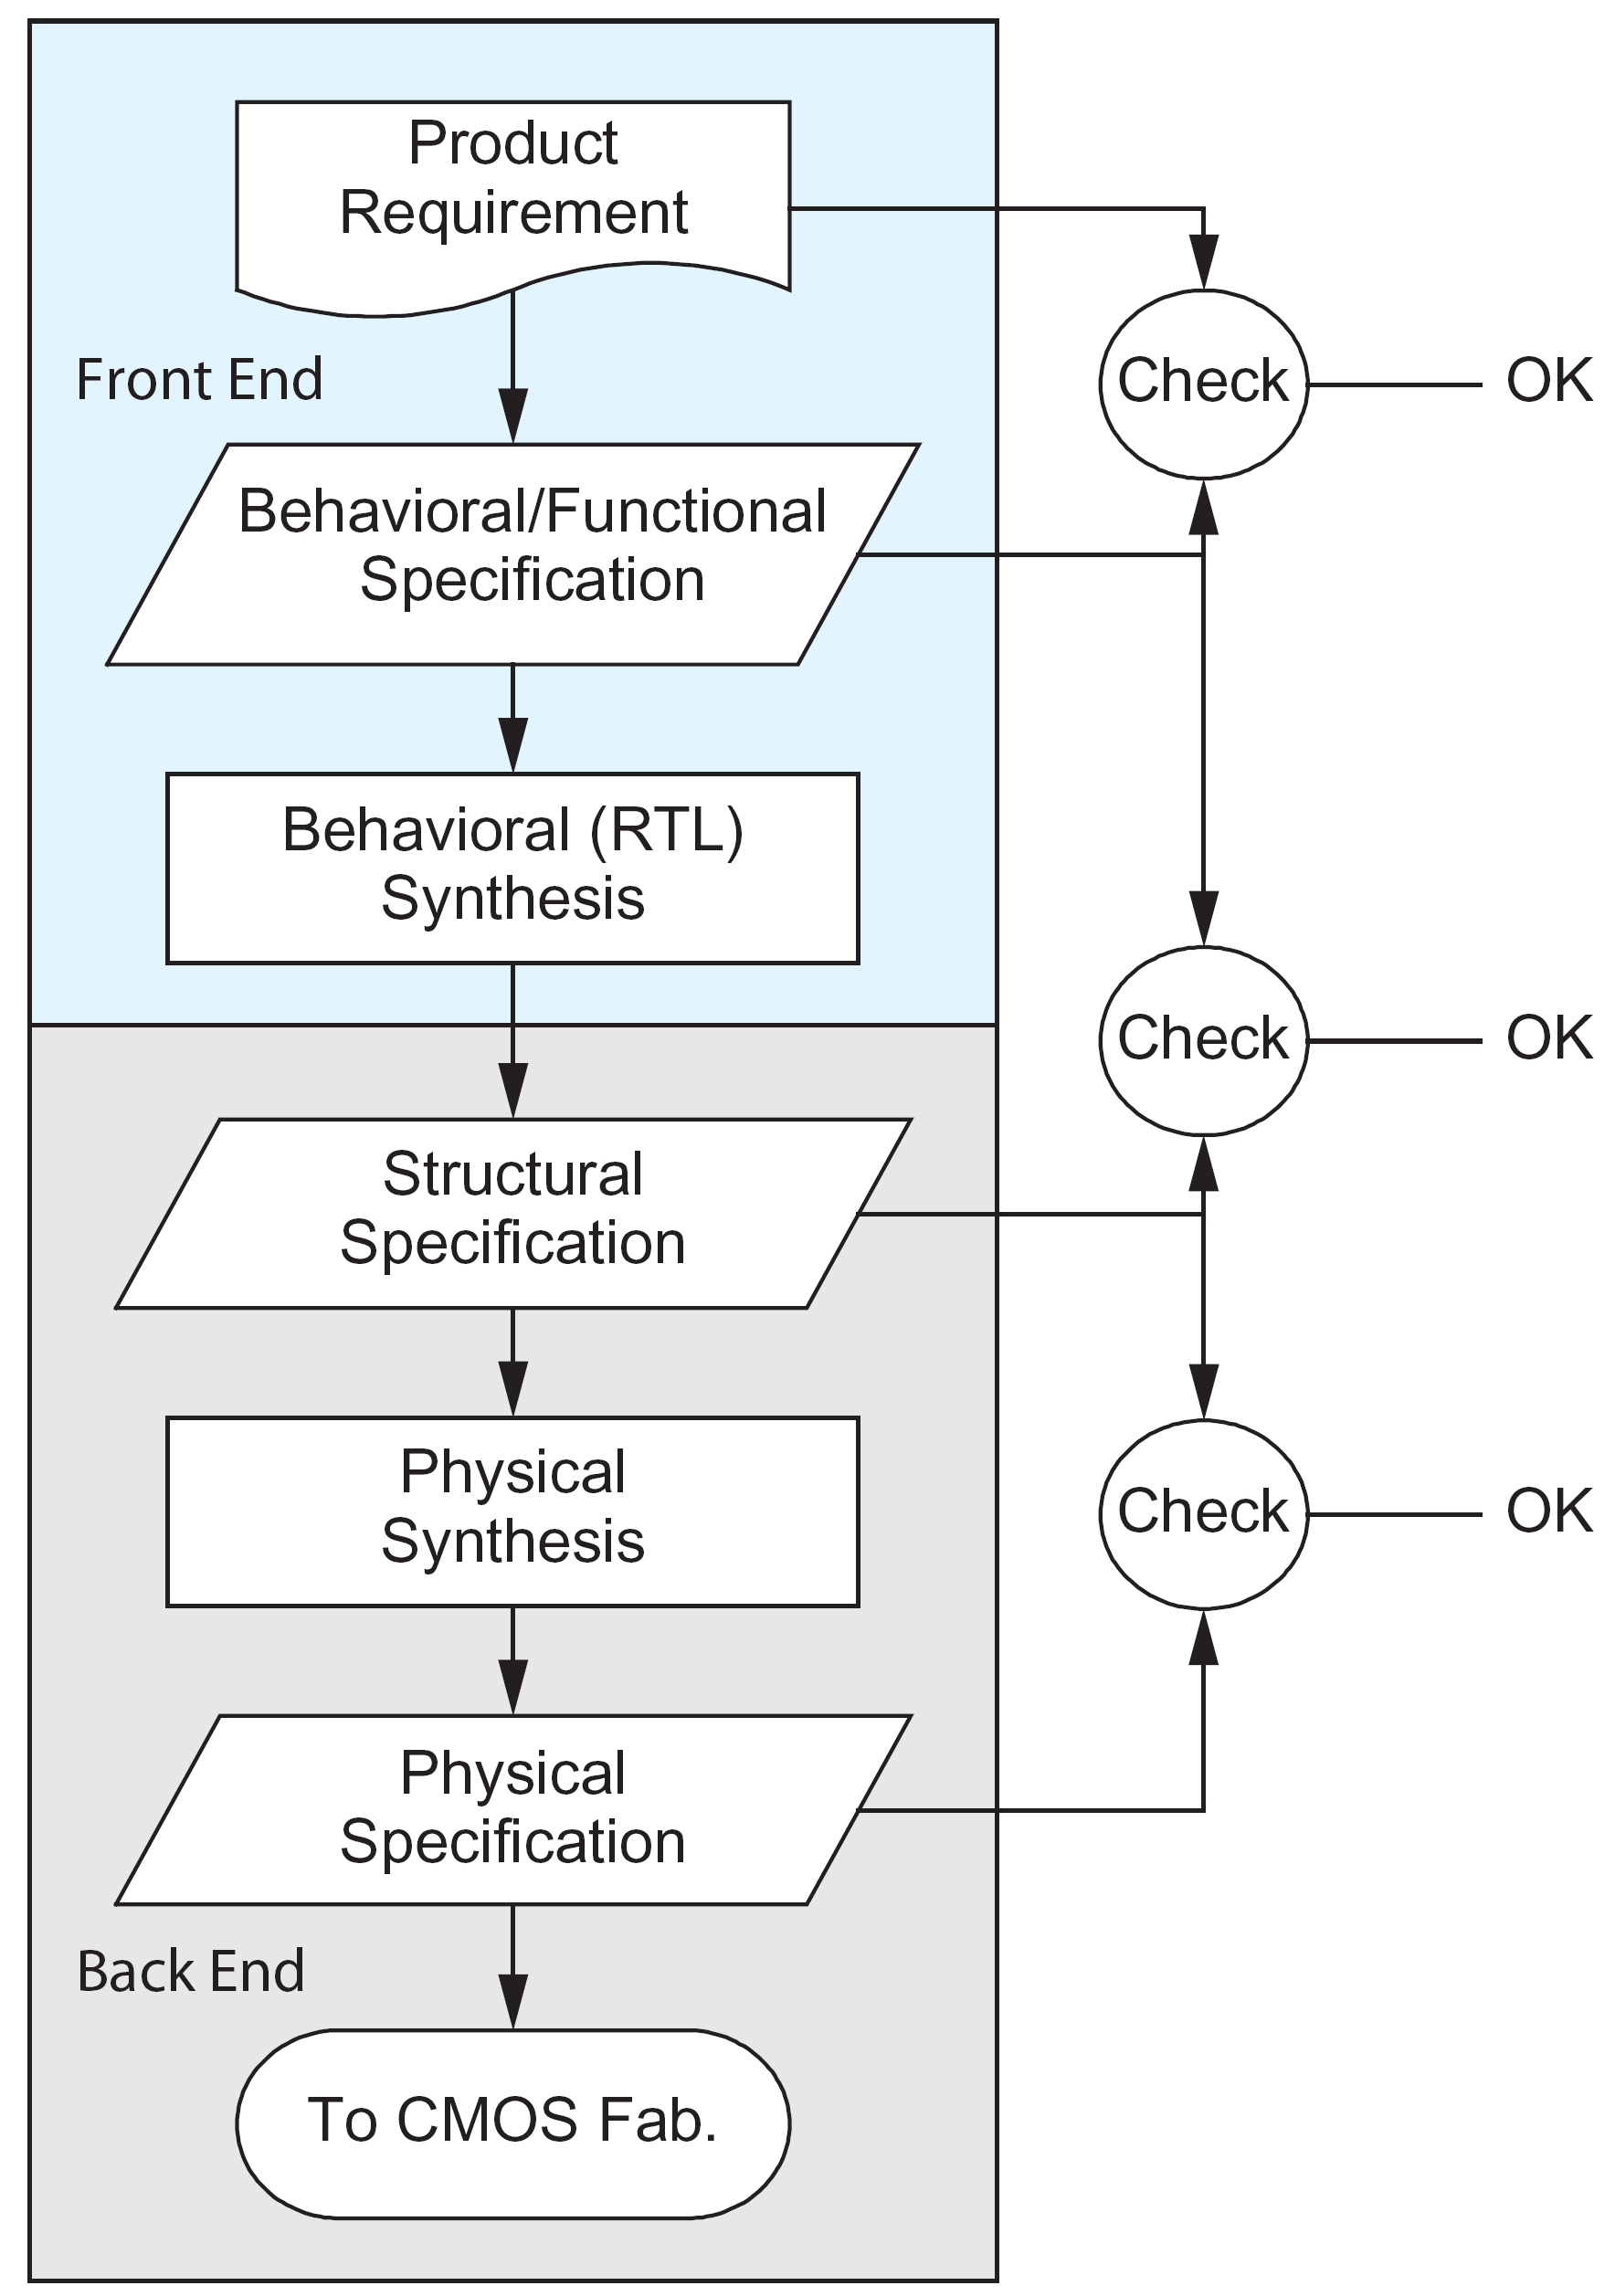
\includegraphics[width=0.25\textwidth]{fluxovlsi.png}
  \caption{Fluxo de projeto VLSI.}
  \label{fig:CMOS2010}
\end{figure}

No processo de desenvolvimento do circuito várias etapas são executadas. Primeiro, há a simulação comportamental para verificar se o circuito descrito em VHDL atende às expectativas, utilizando um \textit{testbench} em VHDL e a ferramenta Cadence NCLaunch. Em seguida, ocorre a síntese lógica, onde a partir do modelo comportamental, utiliza-se a ferramenta Genus para criar um modelo RTL com células padrão de tecnologia específica, considerando restrições de área, frequência e consumo de energia. A síntese gera dois arquivos: um com componentes e conexões, em Verilog, e outro com informações de atraso no formato SDF. A simulação pós-síntese é realizada para validar o netlist gerado usando o mesmo \textit{testbench} da simulação comportamental. Em seguida, na etapa de PAR, o layout é criado posicionando as células e realizando as conexões entre essas células, utilizando a ferramenta Innovus. Por fim, na simulação pós-PAR, o circuito é simulado considerando as resistências e capacitâncias parasitas. Cada etapa é fundamental para garantir o correto funcionamento do circuito.  